% !TEX root = thesis.tex

\section{Evaluating Social Signal Prediction}
\label{section:evaluation}
The output of social signal prediction should satisfy two core requirements: (1) The predicted signals should be within a feasible human motion space showing realistic human motions (realistic motion requirement), and (2) The predicted signals should follow the social rules, spatially and temporally responding to the behaviors of communication partners (social motion requirement). However, it is challenging to qualitatively evaluate these requirement, because there is no objective metric to measure ``realistic" or ``social" behaviors. %The ``realistic motion" requirement can be considered as a necessary condition for the ``social motion" requirement, because non-realistic motion is not acceptable and cannot be suitable to social situations. But it is not sufficient, because realistic jogging motion, satisfying the first condition

Notably, the L2 distance between the predicted signals and ground-truth may not be a good metric because it does not assume diverse possible solutions. Given the same input, human behavior can be still acceptable, but these are penalized if it is different from the ground-truth motion. Due to the reason, L2 metric favors the mean of the data distribution, although it is qualitatively far from expected output. Similar issues have been discussed in human motion forecasting area~\cite{mnih2012conditional, Fragkiadaki_2015_ICCV, jain2016structural}, since there can be diverse possible human motions given a history of input motion. Due to the issue, the area mainly focuses on short-term forecasting (at most several seconds).


In this work, we present a new approach to better evaluate social signal prediction results. We found that for some subpart the L2 distance is reliable, showing that a lower error means a better quality. Classifying speaking status is an example of it. However, if the dimension of the output signals is high, such as body motion, the L2 metric does not consistent to the actual quality of the output. Our idea is evaluating the social signal prediction output by transferring it into easier signal space. As an example, we use our model that regresses speaking status given body motion, and the quality of the body motion is evaluated by computing the accuracy of the speaking status. Speaking signal in our social scenario is an important social cue, which is mainly related to the turn taking rule of communication, and this metric only penalizes such properties. Although this metric is not ideal due to the imperfection of our speaking status regressor, we found that this metric provide a consistency to the qualitative performance of the output. The pipeline of this metric is shown in Figure~\ref{fig:evaluation_bySpeakclass}.


%Good metric is also closely related in training a better model, because the metric can be directly used as a loss function in learning stage. for loss function in the neural network architecture. This is one of the biggest challenging in evaluating the performance of the social signal prediction, and it also related to the loss function in training our models.





%penalize the realist signals if it is deviated from the ground-truth. As an example, in our in synthesizing body gestures, a mean of the entire pose distribution shows very competitive L2 errors compared to predicted output, although qualitatively the mean pose does not satisfy either requirements. Similar issues have been discuss in the forecasting single person's human motions~\cite{mnih2012conditional, Fragkiadaki_2015_ICCV, jain2016structural}. It should be noted that the same metric is also used in training models (e.g., neural network), which makes the output of the model converges to the mean pose in the end. 




%The work in forecasting motion of a single subject focuses on the first requirement~\cite{mnih2012conditional, Fragkiadaki_2015_ICCV, jain2016structural}, and the area suffers from the deficiency of a good evaluation method. The L2 distance between the predicted signals and ground-truth motion is often used


% while the second requirement is more challenging and rarely demonstrated. For example, any arbitrary ground-truth motion capture data can satisfy the first condition (because they are genuine signals of humans), and arbitrary combinations of such motions with smooth transition still can satisfy the condition~\cite{kovar2008motion}, but the second condition can be achieved by properly modeling social communication.
%
%Both requirements are hard to be evaluated.
%
%Good metric is also closely related to learining better model, because the metric can be directly used for loss function in the neural network architecture. This is one of the biggest challenging in evaluating the performance of the social signal prediction, and it also related to the loss function in training our models.
%
%
%We found for some subpart of signals, this L2 metric provided consistent output as in qualitative evaluation, for example, in speaking classification and social formation estimation. They are hard to be applied for more high dimensional signal such as body signal. 
%
%
%
%We can use a human manifold space to evalute the first requirement. If output is far from this manifold space, then we can consider they are less realistic motion; that is the distance between the projected point to the original signal would be an evaluation metric. However, this requires a well-defined manifold space, which is a challenging issue. Moreover, since our motion output are synthesized by this manifold model, they tend to located in the space already, providing biases in evaluation. This output is discussed in Section~\ref{chapter:manifold_metric}. 
%
%The second requirement is very challenging without objective way to measure, due to the inherent diversity of human behaviors. Given an input signals of others, there could be several possible reaction of humans, which all can be possible solution, if it is within our social norms. A common evaluation metric, L2 distance, may penalize the realistic motion if it is far from the ground truth motion measured in our system. 
%
%We present an indirect method as a way to quantitatively measure the quality of prediction output. We use our trained network which takes body motions and produces signals which can be more reliably evaluated (e.g., speaking signals). Since the timing of speaking is closely related to the social interaction (turn taking), it can be used to evaluate the social requirement. We found that this method shows a reasonable output by penalizing the mean pose and favor the qualitatively better estimation output. This output is discussed in Section~\ref{chapter:classifier_metric}. 



\begin{figure}
	\centering       
	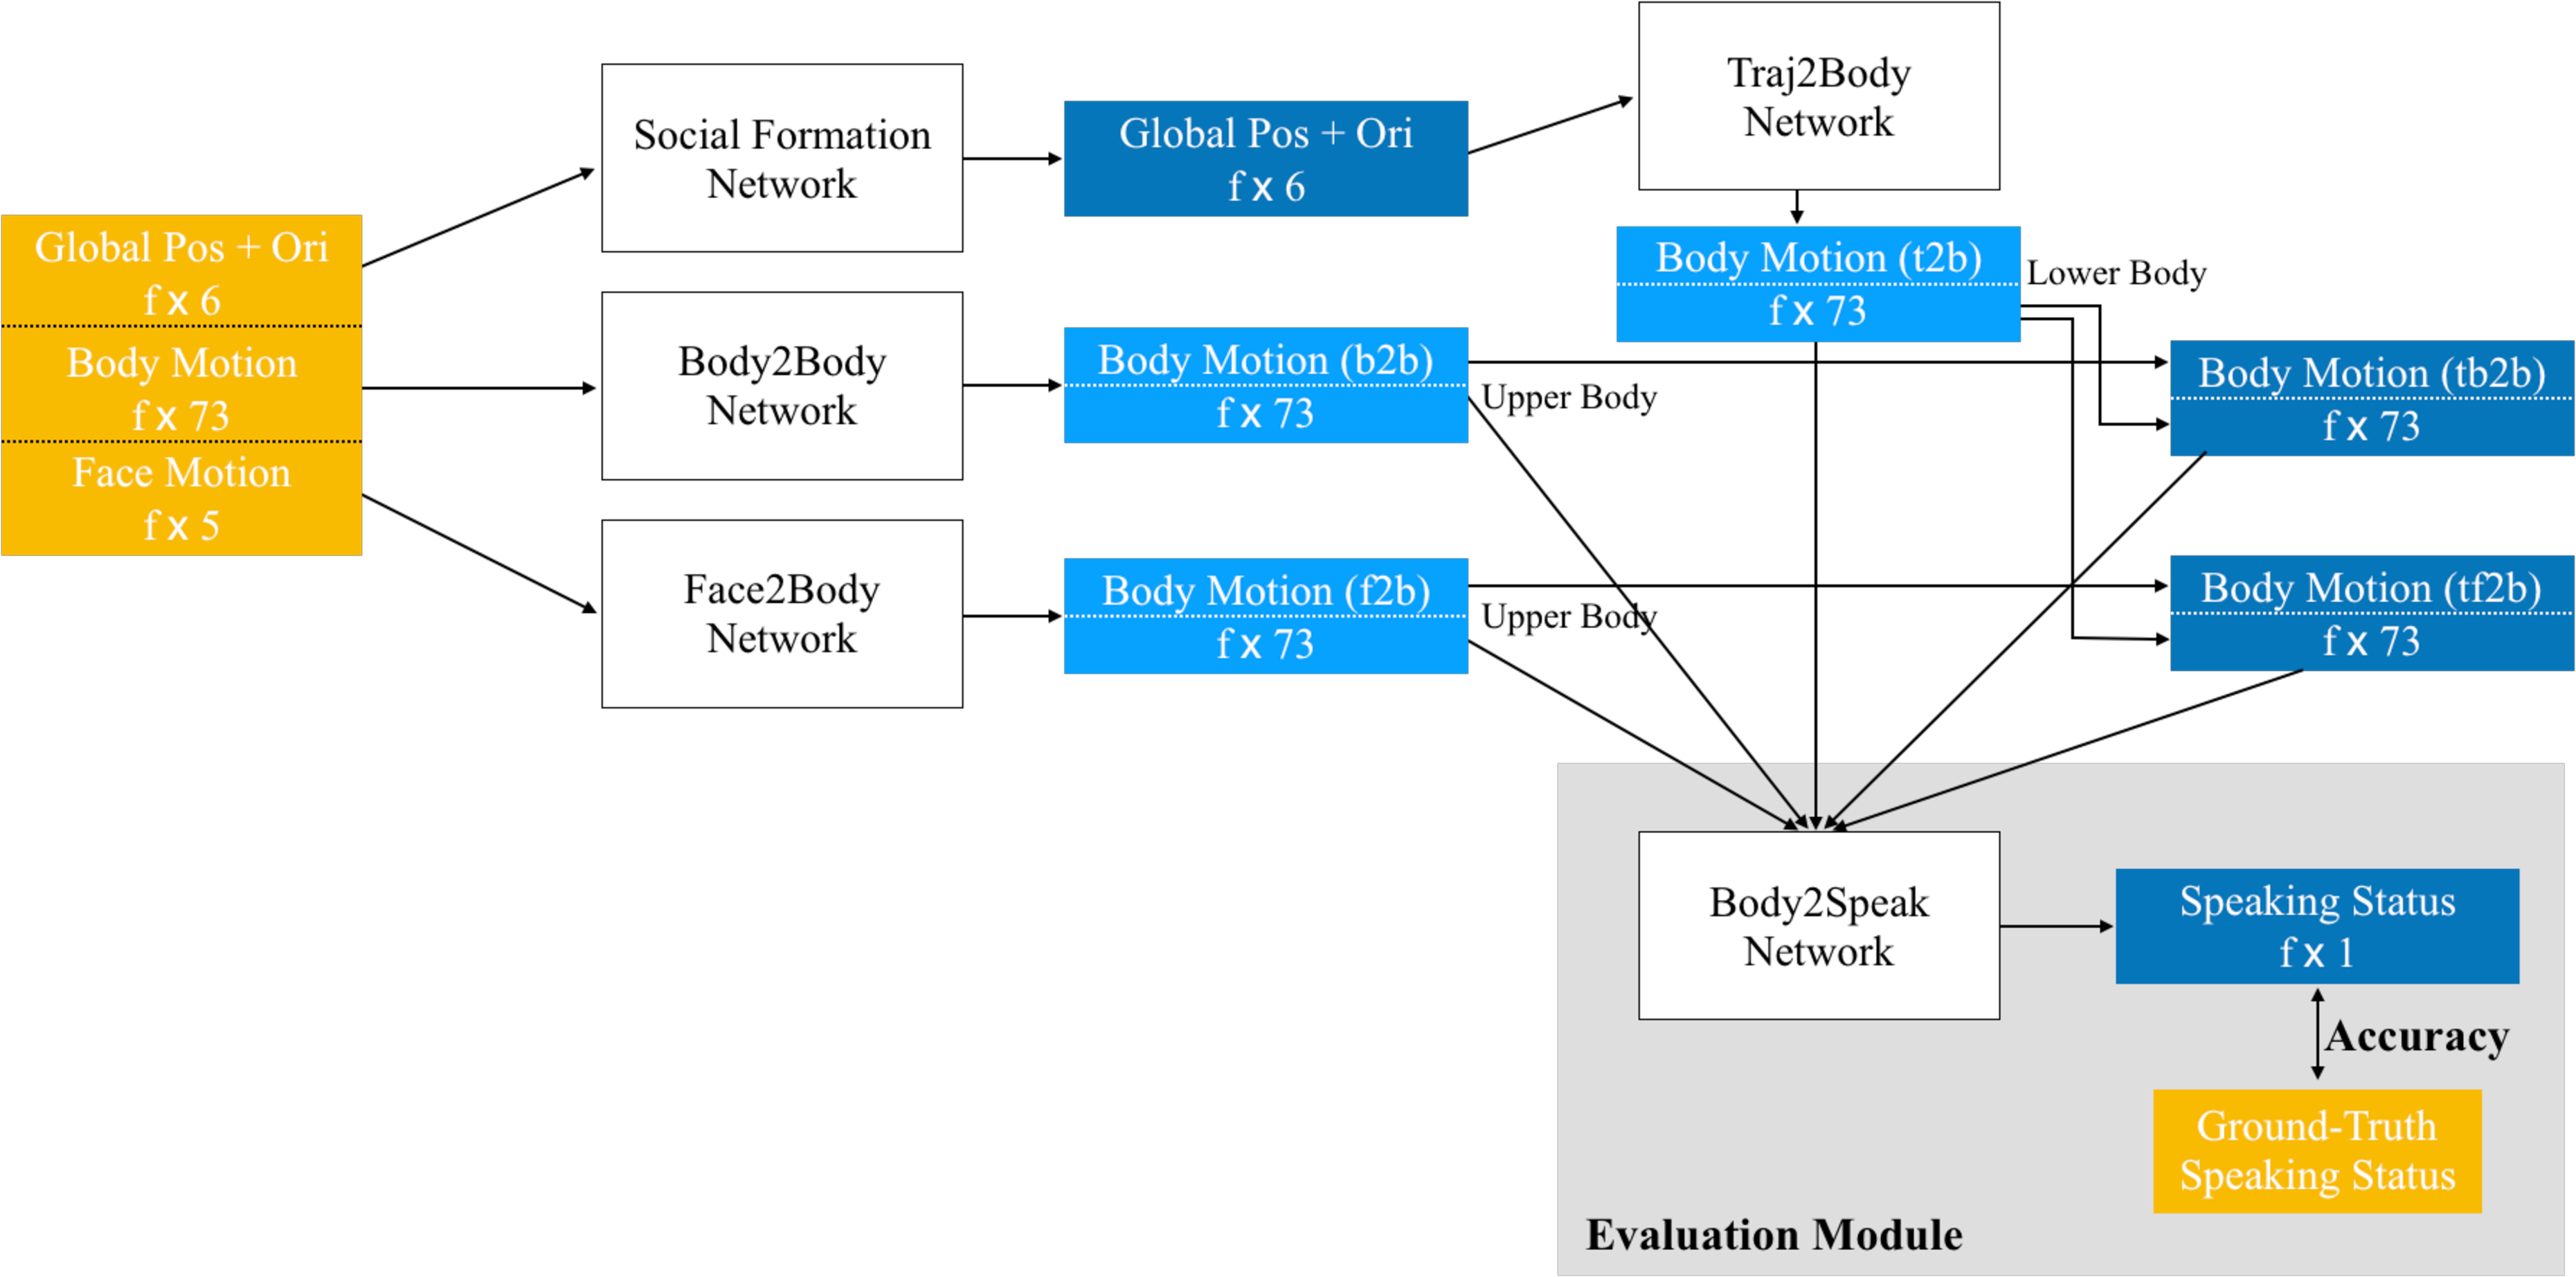
\includegraphics[ width=0.8\linewidth]{ssp_fig/evaluation_pipeline.pdf}
	\caption{Evaluating body motion prediction by speaking classification} 
	\label{fig:evaluation_bySpeakclass}
\end{figure}


\section{Results}
In this section, we show various experimental results by modeling the dynamics among social signals. The core direction in performing this experiments is to explore and compare the correlations of diverse behavioral channels observed in genuine social communications. We leverage the wide spectrum social signal measurements of the Haggling dataset, and build neural network models to predict speaking status, social formations (positions and orientations), and body gestures of the target person, by using different input sources. 

\subsection{Pre-processing Haggling Data}
Given the motion data of the Haggling games, we first annotate the start and end time of the game, where start time is decided when the social formation is built and the end time is defined when the social formation is broken. We crop out the motion dataset based on this start and end time, so that we ignore the time while subjects enter and exit the capture space. For each haggling game scene we also annotate the roles in the game, buyer, left-seller, and right-seller, where the left and right are determined in the buyer's view point. In our experiment we specify that the left seller is our target person and predict the social behavior of these subjects. Following the work of~\cite{holden2016deep}, we re-target the motion data to a standardized skeleton size to remove size variation from the body skeletons. We also synthesize footstep signals and decouple the body motion from global translation and orientation using the method of ~\cite{holden2016deep}. Finally we divide the dataset into 140 training sets and 40 test sets. However, since there exist sequences where the reconstruction errors are severe for some frames, we select only 79 training sets and 28 testing sets which are manually verified to be error free. Although our dataset captures face and body signals, we do not include these data in our current experiments. 


\subsection{Verification of Proxemics}
An interesting experiment is to consider the well-know theories in psychology again using the new data we collected in our sensor system. Our dataset has the measurement of fully voluntary motions (including the position and orientation of groups) of interacting people, and enables us to revisit the well-known proxemics theory~\cite{Hall66}. We first compute the average distance between a pair of subjects: (1) buyer and right sellers (B-RS), (2) buyer and left seller (B-LS), and (3) left seller and right seller (LS-RS). The results are shown in Table~\ref{table:proxemics_comp}. We found that the result approximately follows the social distance categories defined in the Hall's categorization~\cite{Hall66}. The distances among sellers are within the close phase of social distance ranges (from 120-210 $cm$) and the average distance among sellers and buyers are within the far phase of social distance (from 210 to 370 $cm$) in \cite{Hall66}. To analyze the shape of the social formation, we plot the average formation of games in a person-centric coordinate by a buyer. The results are shown in the Figure~\ref{fig:socialgeo_distribution}, showing that the formation is often similar to isosceles triangles with relatively far distances between a buyer and two sellers than the distance between sellers. 


\begin{table}[t]
	\centering
%	\footnotesize
	\caption{Average distances (cm) between subjects. B, RS, and LS denote buyer, right seller, and left seller respectively.}
	\label{table:proxemics_comp}
	\begin{tabular}{c| c| c| c| c}
		\hline
		%Types & Avg. dist. (cm) & Std.(cm) & Min dist. (cm)  & Max dist. (cm)\\
		& Avg. dist. & Std. & Min & Max \\
		\hline
		B-RS & 148.11 & 27.26 & 99.03 & 265.52 \\
		\hline
		B-LS & 151.45 & 29.62 & 104.24  & 284.85 \\
		\hline
		LS-RS & 124.13 & 24.05  & 77.70  & 206.26 \\
		\hline
	\end{tabular}
\end{table}

\begin{figure}
	\centering       
	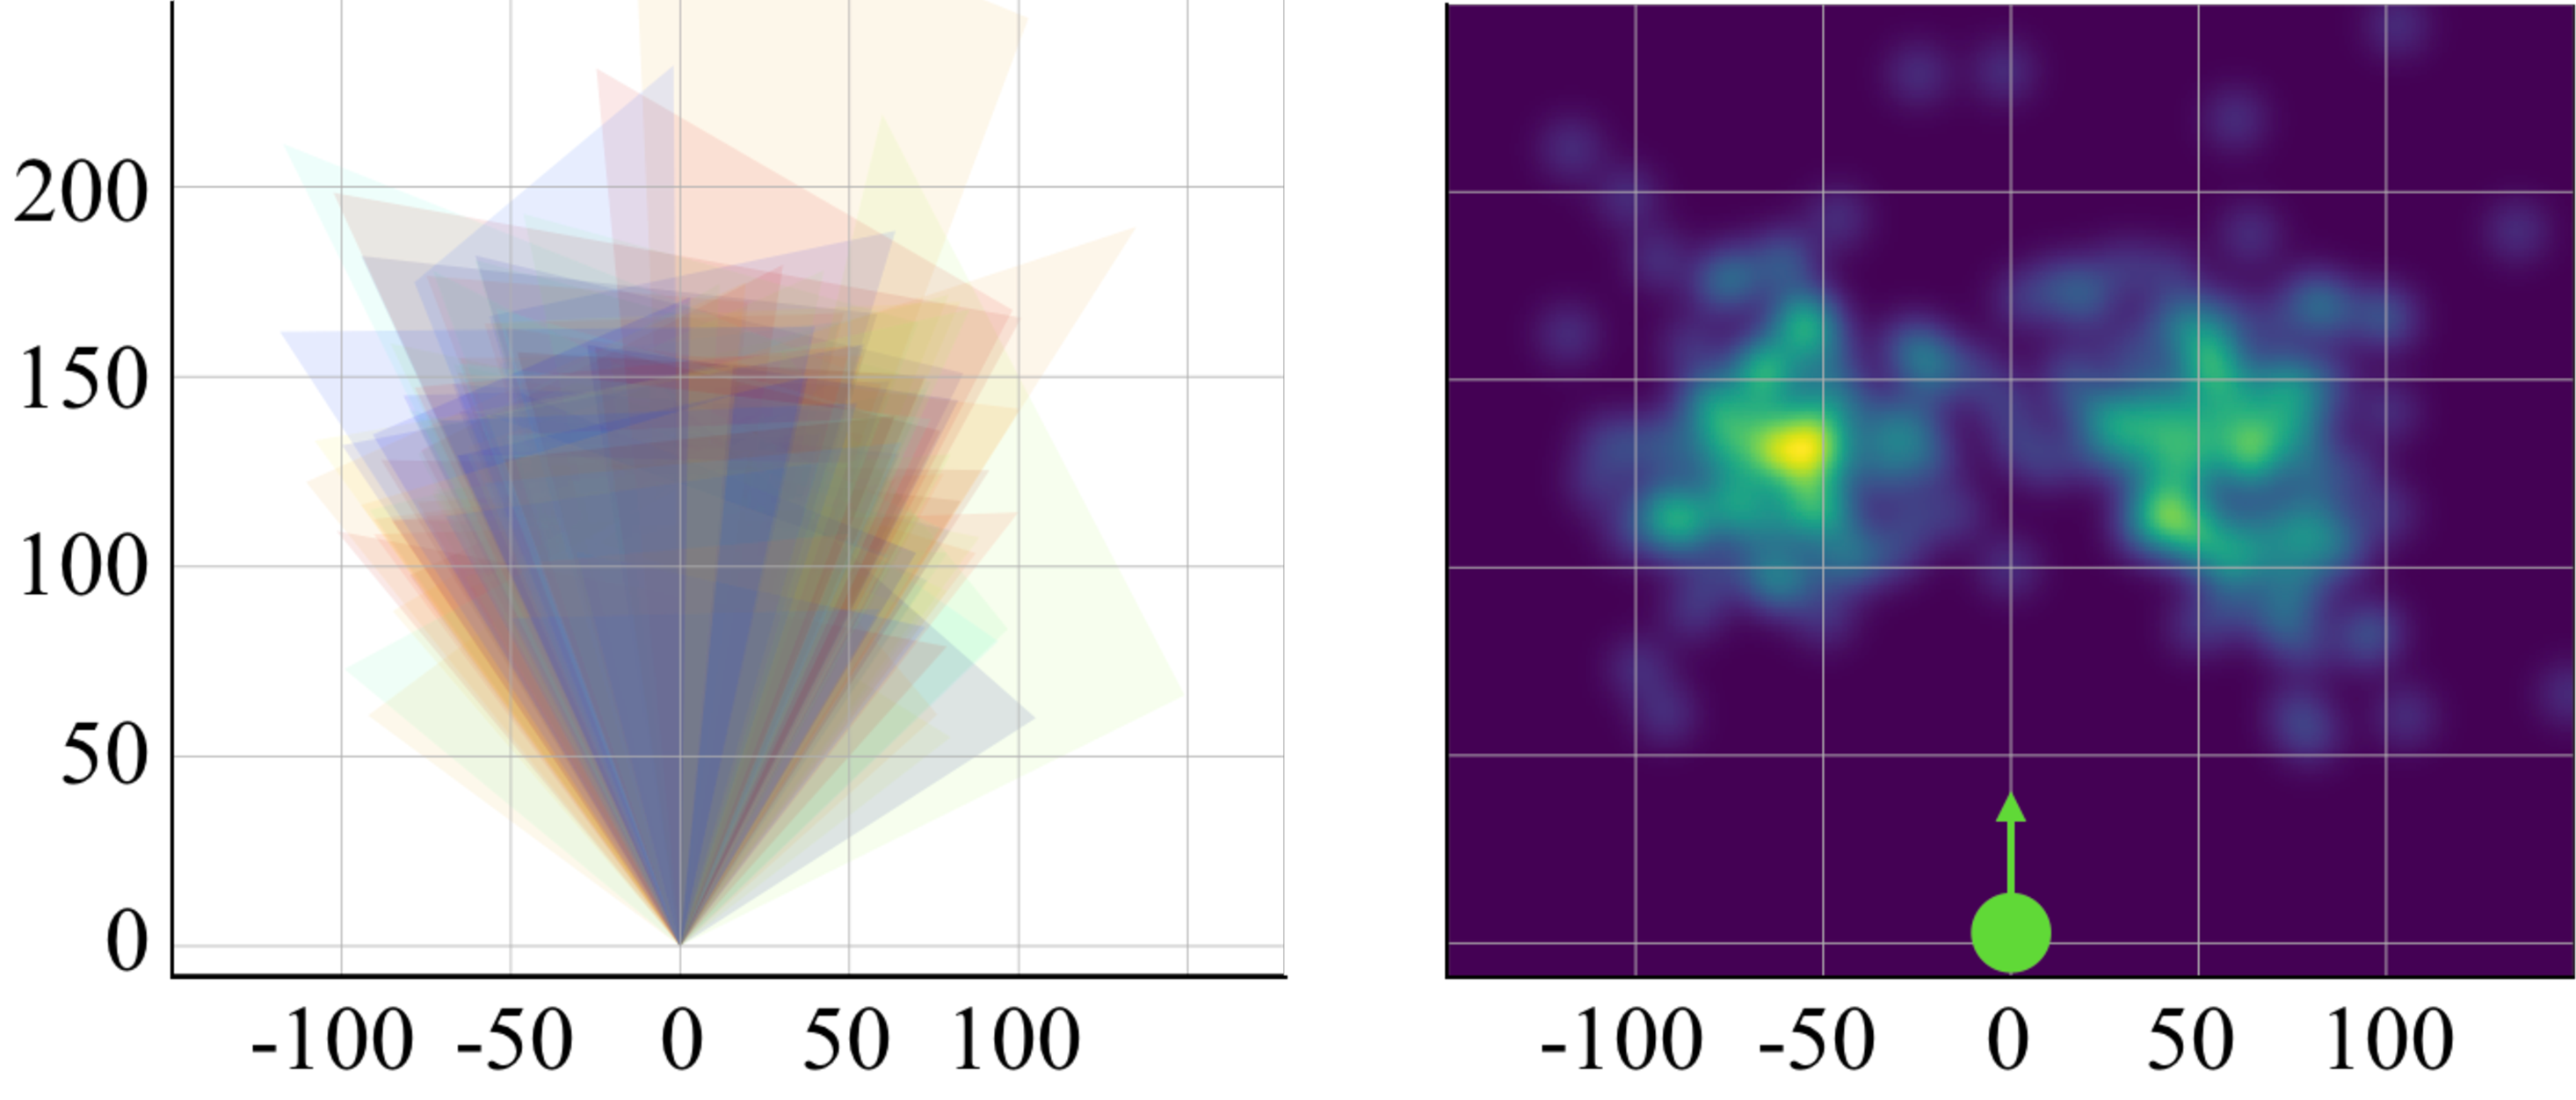
\includegraphics[ width=0.8\linewidth]{ssp_fig/haggling_proxemics_stat.pdf}
	% 	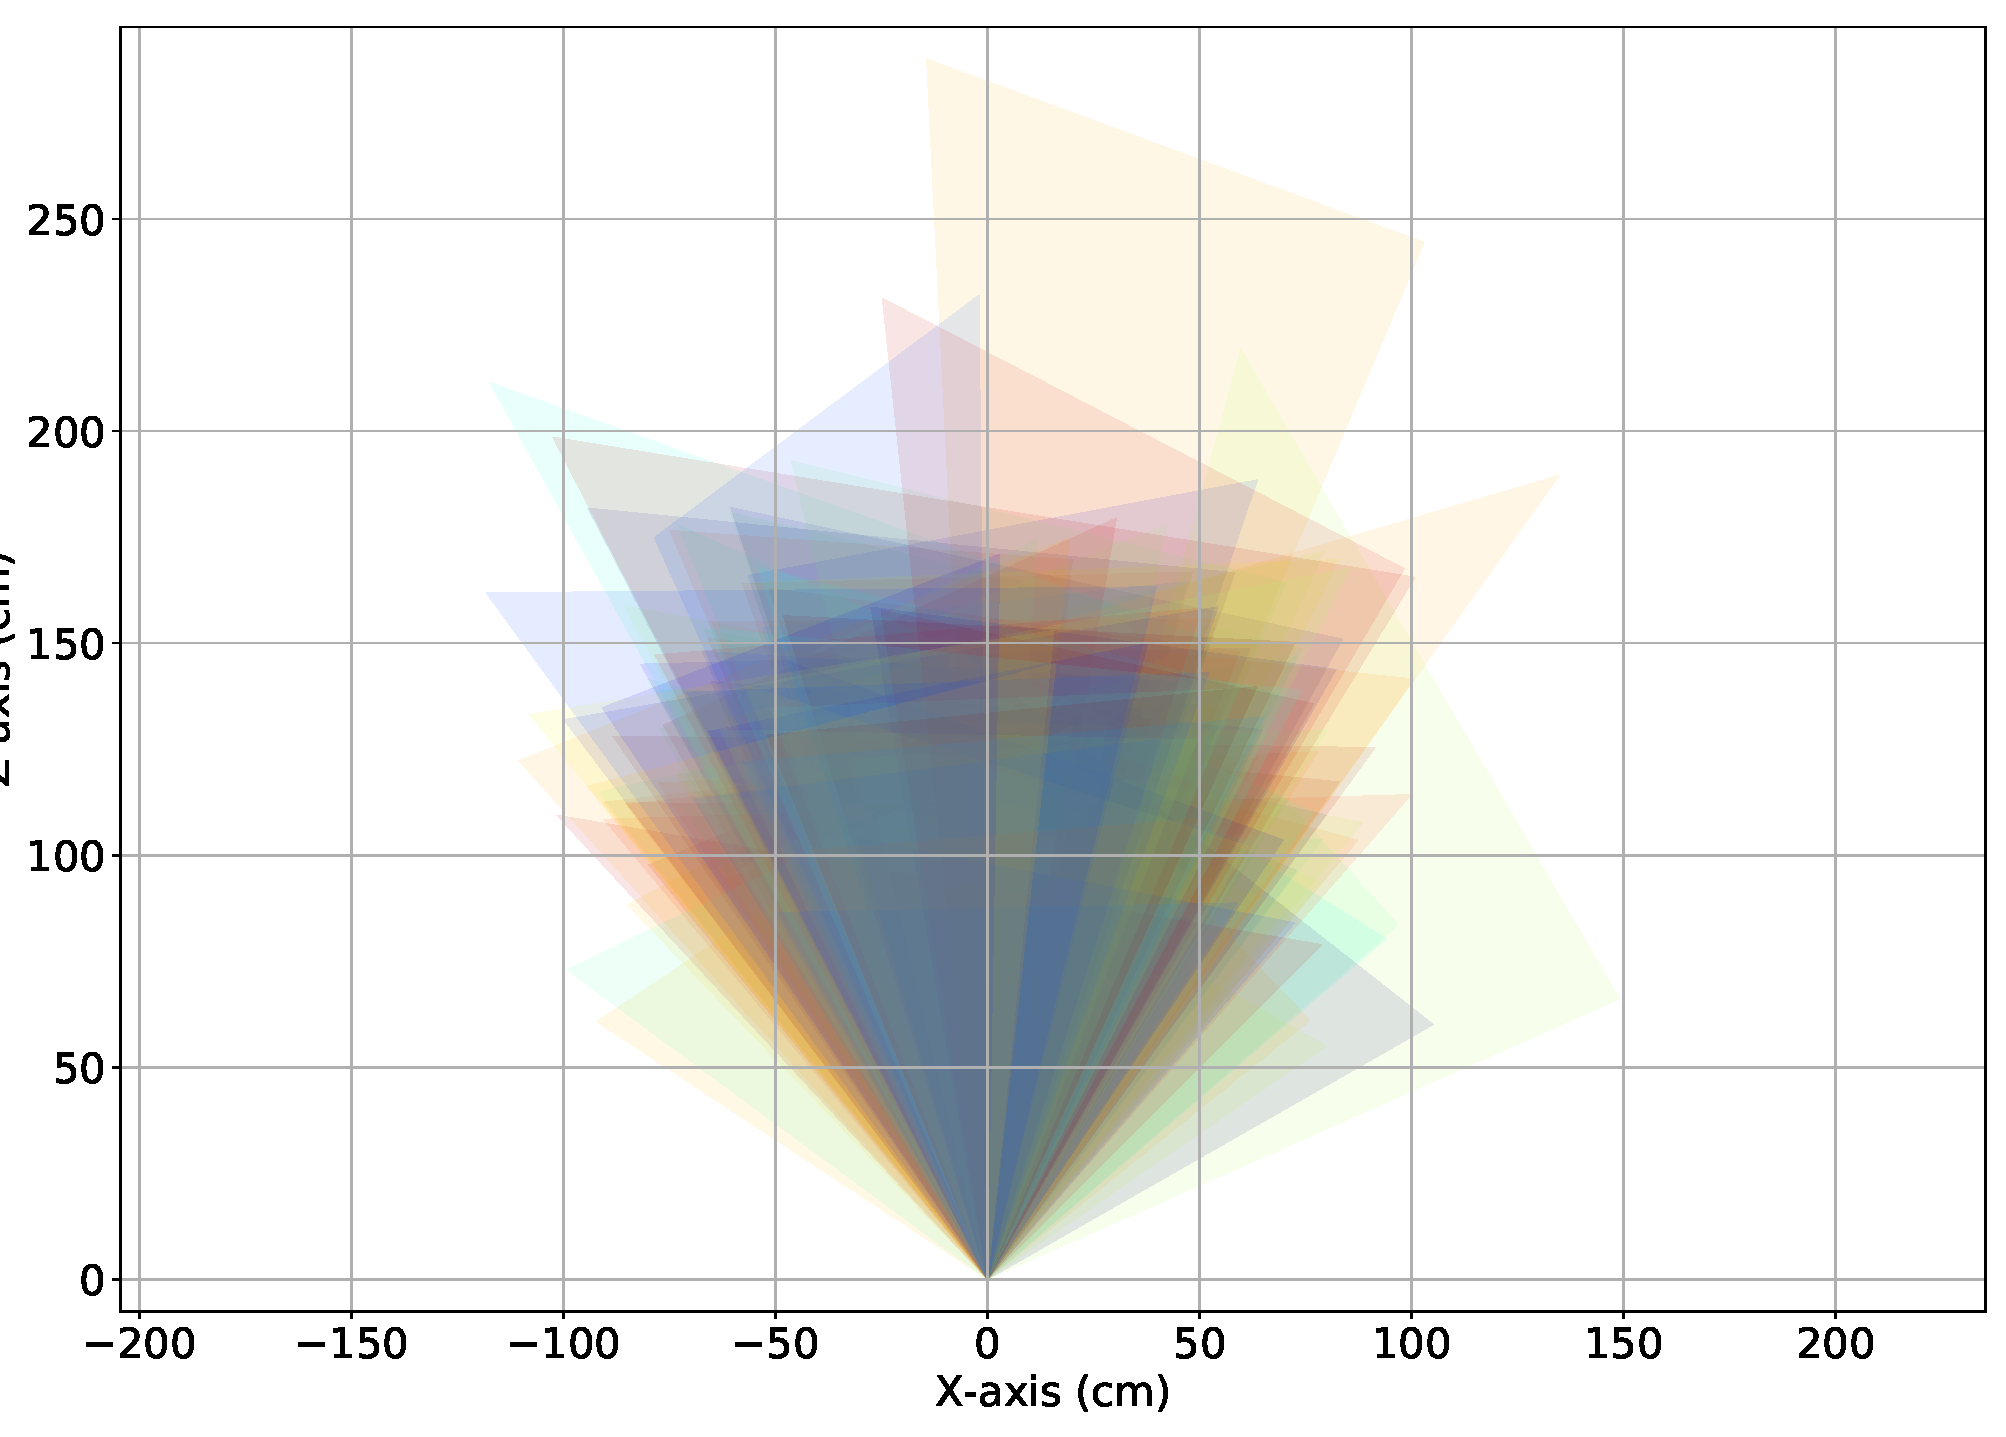
\includegraphics[trim=120 0 120 0,clip, width=0.45\linewidth]{plot/haggling_proxemics_polygon.pdf}
	% 	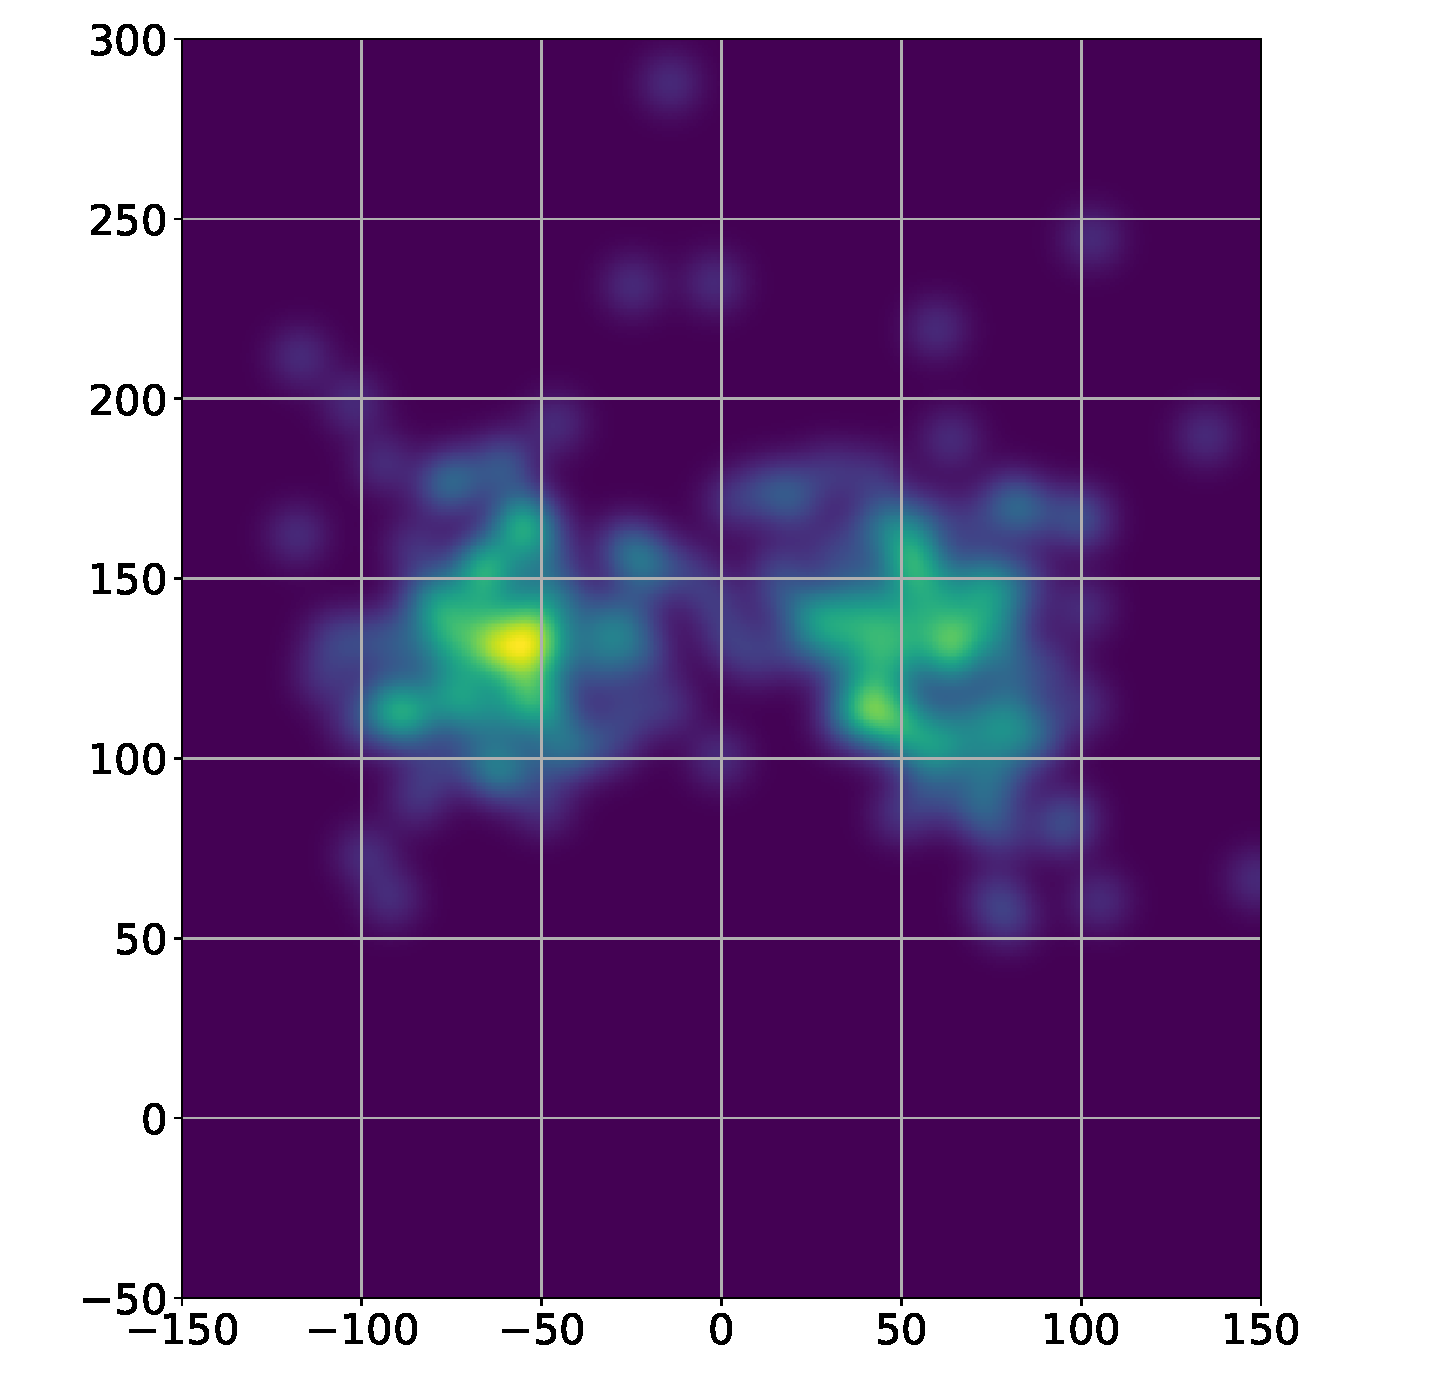
\includegraphics[width=0.45\linewidth]{plot/haggling_proxemics_heatmap.pdf} 
	%	\subfigure[TrajCompares]{\label{Fig:asso_traj}\includegraphics[width=0.5\textwidth]{img/trajCompare}}   
	\caption{Visualizing social formations in the haggling sequences as triangles (left) and a heat map (right). The formation is normalized w.r.t the buyer's location, and the green circle on the right shows the buyer location (origin) and orientation ($z$-axis).} 
	\label{fig:socialgeo_distribution}
\end{figure}

% \begin{figure}
% 	\centering       
% 	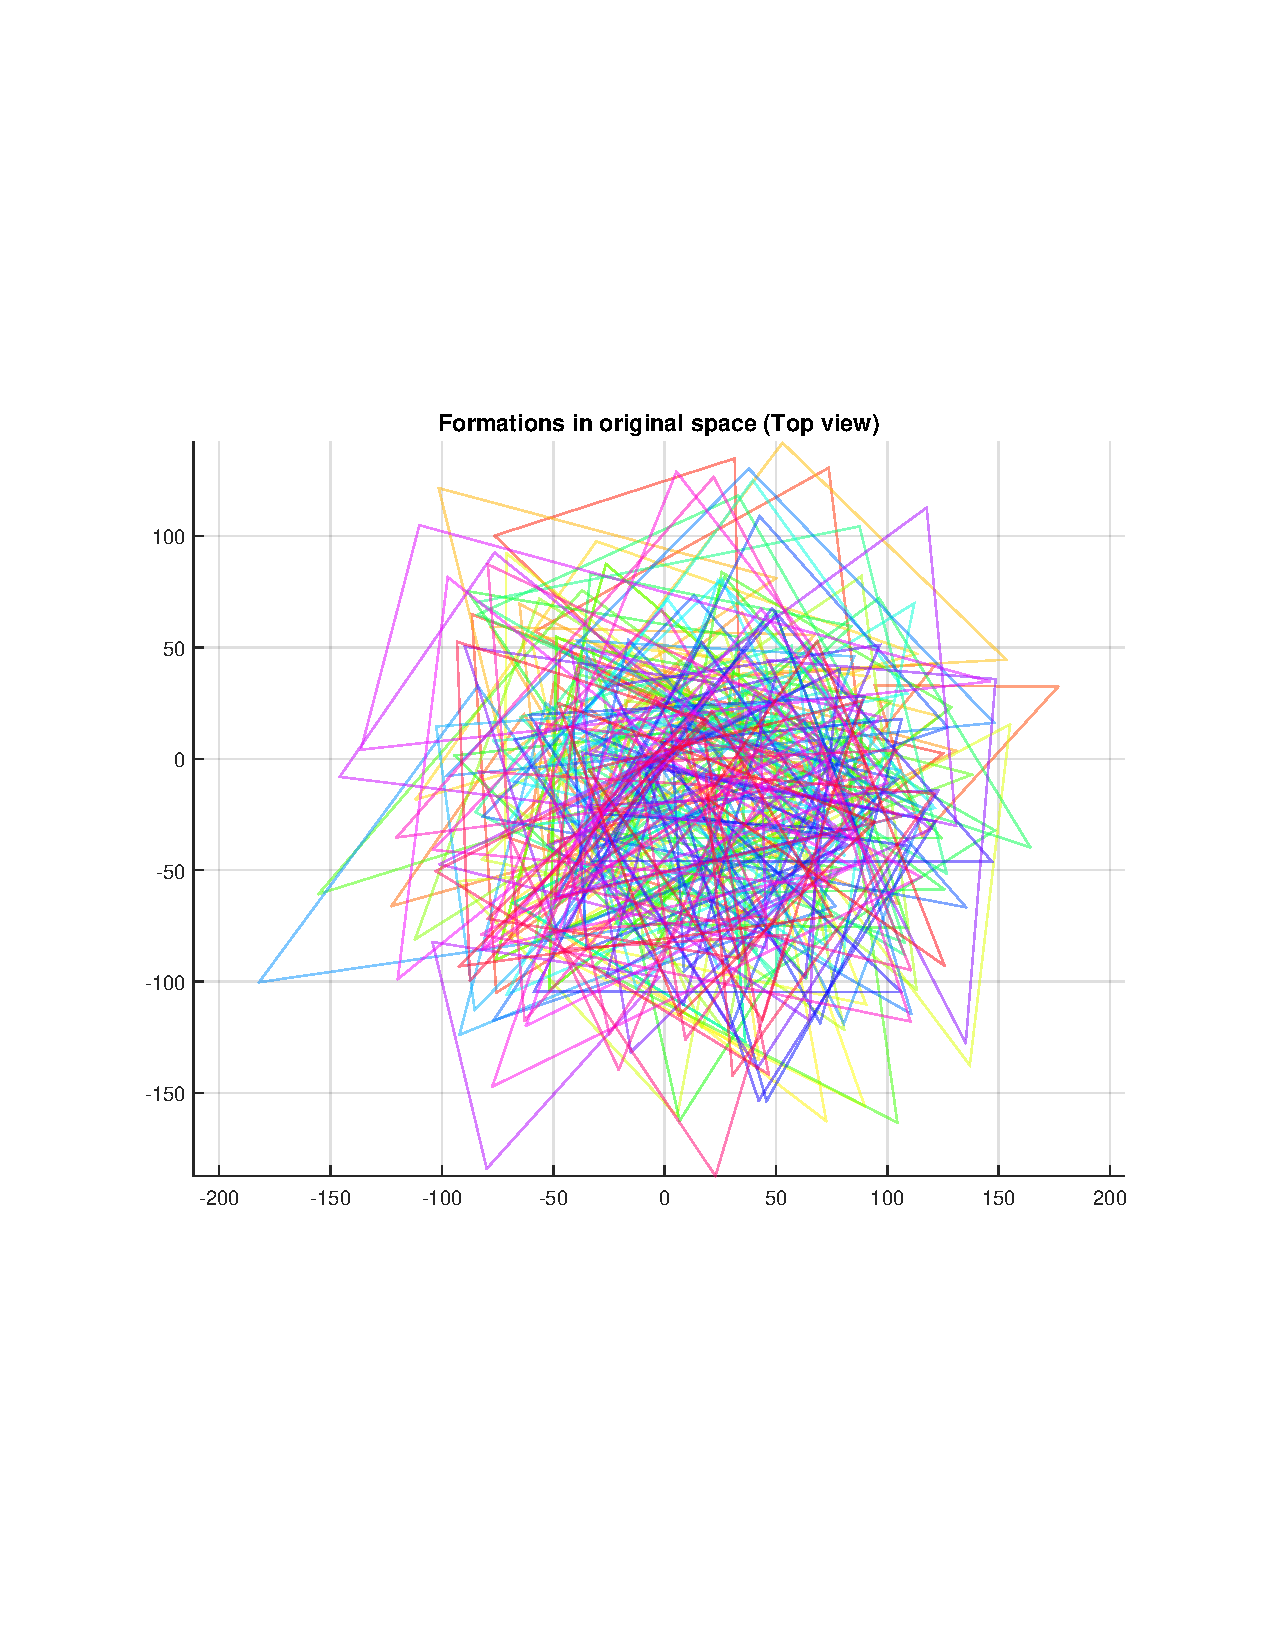
\includegraphics[trim=60 200 60 150,clip,width=0.32\linewidth]{fig/originalTri}
% 	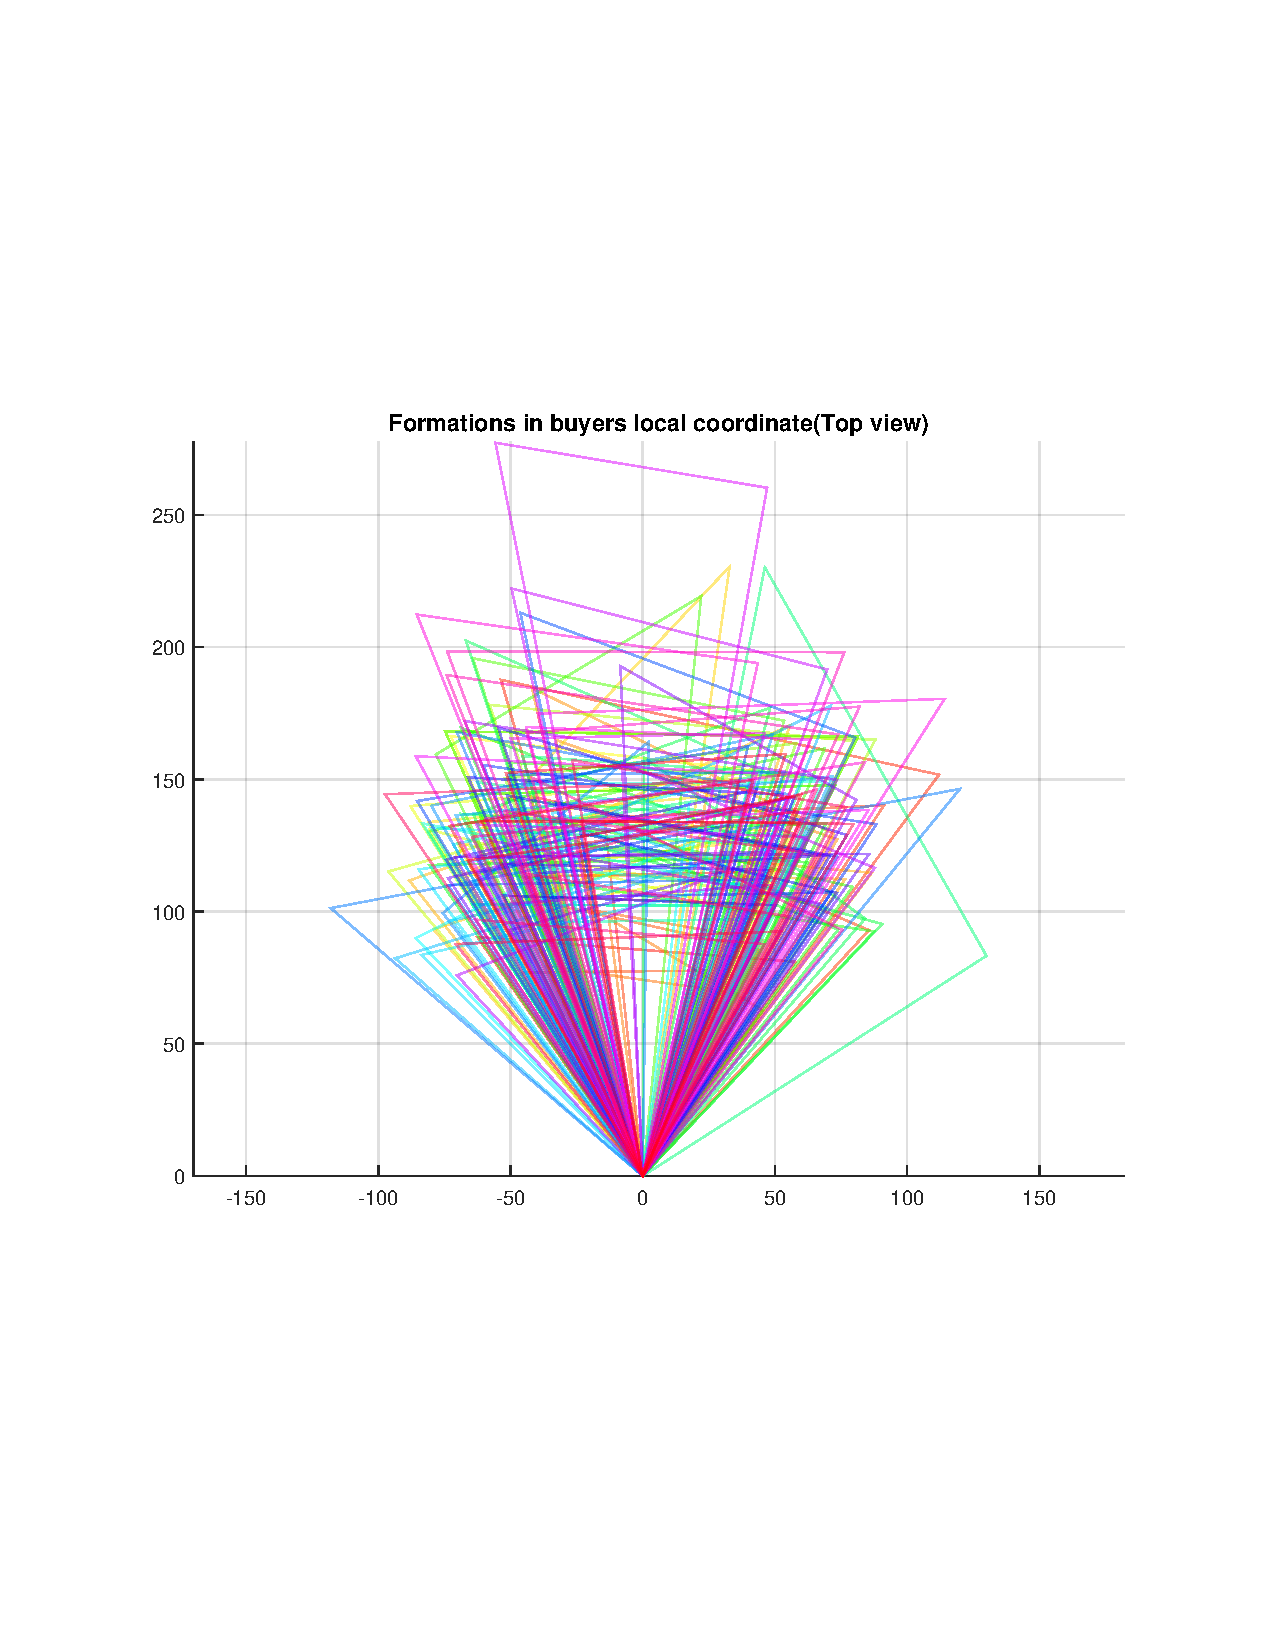
\includegraphics[trim=60 200 60 150,clip,width=0.32\linewidth]{fig/buyersTri} 
% 	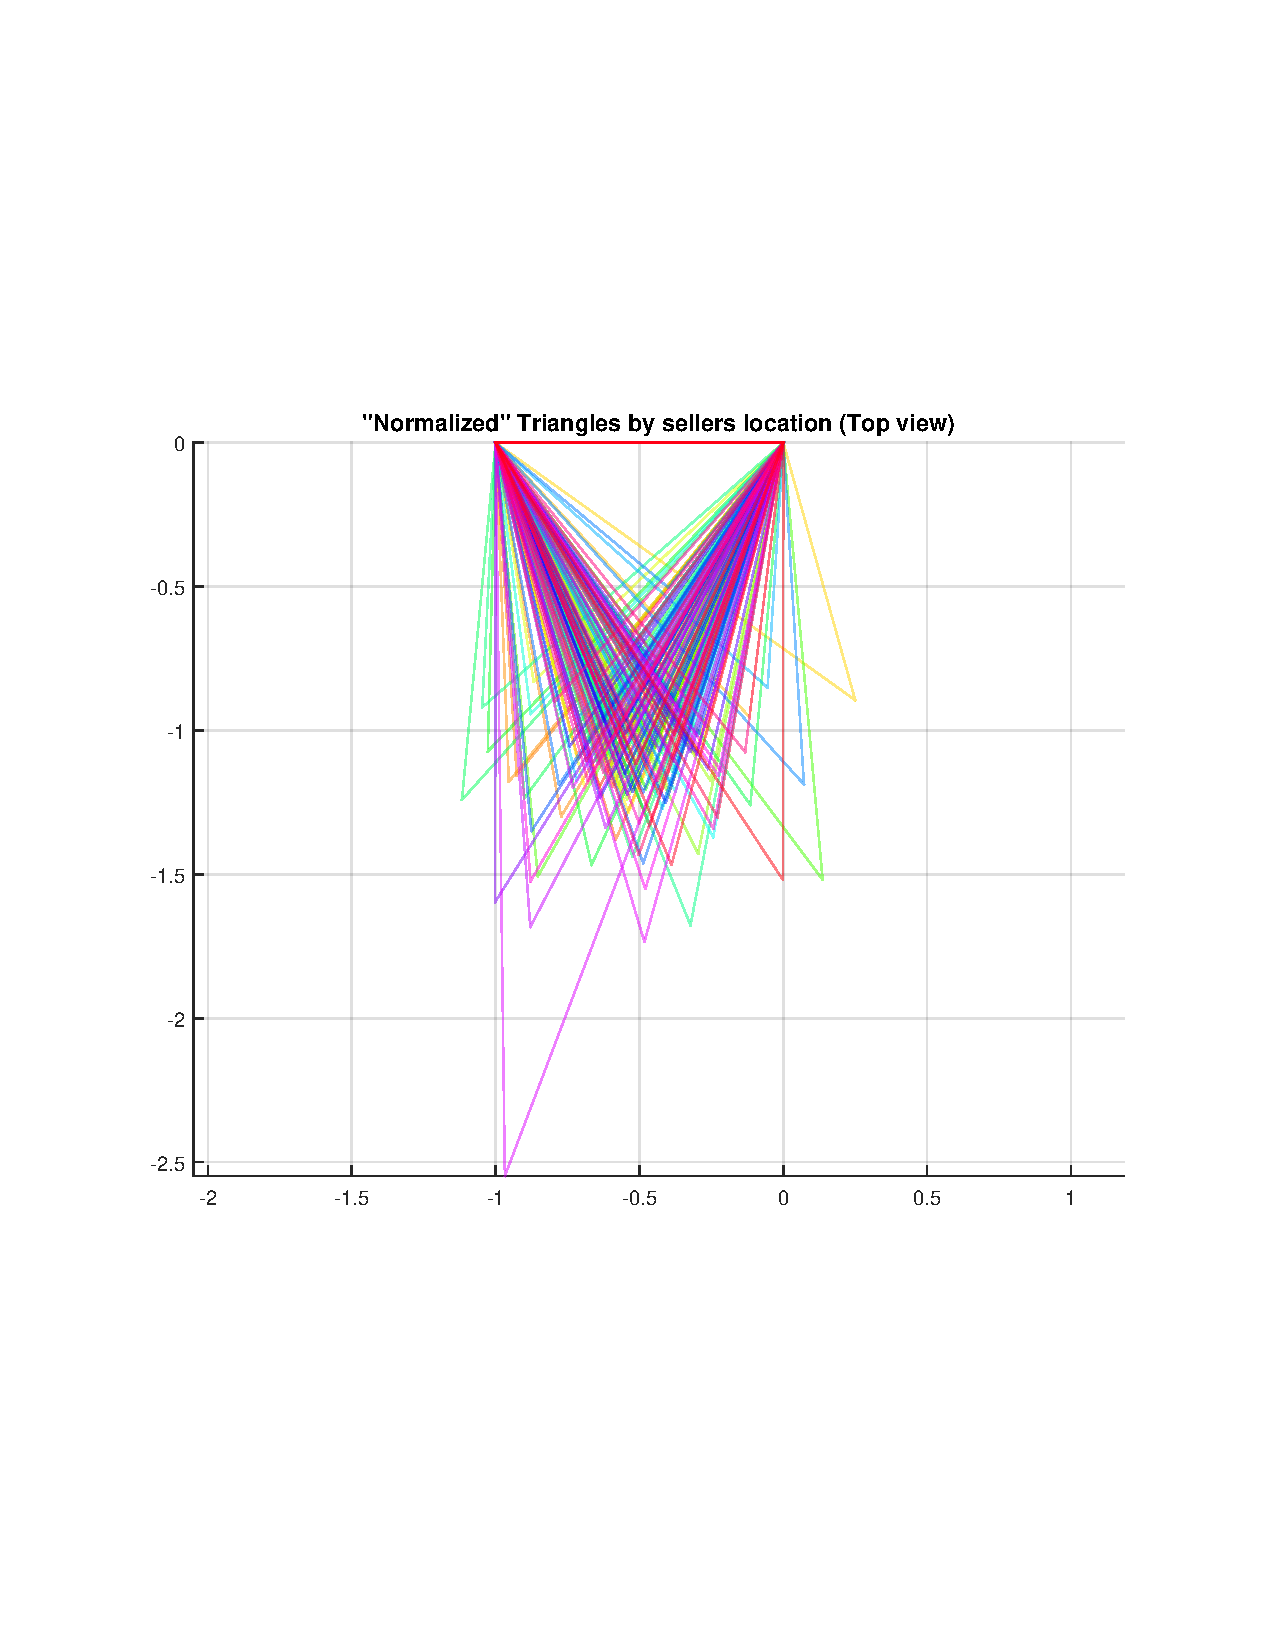
\includegraphics[trim=60 200 60 150,clip,width=0.32\linewidth]{fig/normTri} 
% 	%	\subfigure[TrajCompares]{\label{Fig:asso_traj}\includegraphics[width=0.5\textwidth]{img/trajCompare}}   
% 	\caption{Social formations in three different representations. (a) Global coordinate; (2) Person-centric coordinate defined by buyers; (3) Normalized-by-a-pair coordinate system define by two sellers} 
% 	\label{fig:socialgeo_distribution}
% \end{figure}

\subsection{Speaking Status Prediction}
We predict whether the target person is currently speaking or not by observing various other social signals in the scene. First, we consider the target individual's own social signals as input. Three different types, facial expressions, body gestures, and both of them, are used to train neural network models separately. We use the same neural network architecture for these models to fairly compare the performance, and mask out if some input signals are used. More specifically, we use the``body2speak" model in \ref{section:body2speak}, by modifying the input dimension into the concatenation of face and body signals (with $5+73$ dimensions). For body only test, we mask out the face signal part in the input with their average values, and do the similar thing if we test the model with face signal only.  The prediction accuracies from these own signals of the target person are shown in the first column of Table ~\ref{table:speaking_class}. Facial cues show the strongest correlation with speaking status, presumably due to lip motion. Own body motion also shows a strong correlation. When we use both face and body, it seems like the face signal dominates, showing a similar performance with face only case. 

More interesting experiments is performed by using the other seller's social signals as input to predict the target person's speaking status. Similar three types of social signals are considered. The result clearly shows that there exists a strong link between interpersonal social signals. The other seller's facial motion is a strong predictive cue, which presumably learns the turn-taking property in social communication.% predicting that the target person is speaking if little motion is observed from the other sellers. Other seller's body signals are also very predictive in this task. 

For the sake of comparison, we also test with the social signals of a random person, where the person is randomly selected in the testing set. As expected, the classification performance using a random person's motion as input shows about the chance level (50\%). 

%We compare the binary speaking classification performance . The task is to classify the speaking status of the target person, and we use three different body motion sources: (1) the target person's own body motion, (2) the other seller's body motion, (3) a random person's body motion. As shown in the results, the own body motion has the strongest correlation, but the other seller's body motion is also very predictive, showing that there exists a clear social link during their interaction. As expected, the classification performance using a random person's motion as input shows about the chance level (50\%). For the experiment (3), we use the same network trained for (2), but use the body motion from a subject in some other arbitrary sequence (excluding our current target sequence) as input. Presumably, the classification method using the other person's body signals learns the ``turn-taking" property in the social interaction, and predicts that the target person is speaking if little motion is observed from the other sellers (who would be listening). %This kind of study is important to make machines better understand human social behaviors, and can be facilitated from the data where natural social interactions are captured.  %This kin %shows an interesting insight that the body motions % the strong correlation of social signals can be used as a prior for predicting human behaviors. 
%\begin{table}[t]
%	\centering
%%	\footnotesize
%	\begin{tabular}{l| l| l| l}
%		\hline
%		%Types & Avg. dist. (cm) & Std.(cm) & Min dist. (cm)  & Max dist. (cm)\\
%		Input Signal & Own body & Other seller & Random person\\
%		\hline
%		%Accuracy & 80.34\% & 73.44\% & 53.39\%\\
%		%Accuracy & 76.16\% & 70.33\% & 51.05\%\\       %submitted
%		Accuracy & 80.70\% & 75.30\% & 51.05\%\\       %new
%		\hline
%	\end{tabular}
%	\caption{Speaking Classification Accuracy using different source of body motion signals as input\label{table:speaking_class}}
%\end{table}


\begin{table}[t]
	\centering
%	\footnotesize
	\begin{tabular}{c| c| c| c}
		\hline
		%Types & Avg. dist. (cm) & Std.(cm) & Min dist. (cm)  & Max dist. (cm)\\
		Input Signal Types/Sources & Self signal & Other seller's signal & Random person's signal\\
		\hline
		%Accuracy & 80.34\% & 73.44\% & 53.39\%\\
		%Accuracy & 76.16\% & 70.33\% & 51.05\%\\       %submitted
		Face+Body & 89.13\% & 77.97\% & 49.65\%\\       %new
				\hline
		Face & \underline {\textbf{89.16}}\% & \underline {\textbf{80.21}}\% & 49.64\%\\       %new
				\hline
		Body & 76.69\% & 71.29\% & 50.22\%\\       %new
		\hline
	\end{tabular}
	\caption{Speaking Classification Accuracy using different source of signals as input\label{table:speaking_class}}
\end{table}

\begin{table}[t]
	\centering
	%	\small
	%\caption{Social Formation Prediction Errors (cm) }
	\begin{tabular}{c| c| c| c}
		\hline
		%Types & Avg. dist. (cm) & Std.(cm) & Min dist. (cm)  & Max dist. (cm)\\
		Types & Position & Body Orientation & Face Orientation\\
		\hline
		PosOnly & 29.83 (13.38) & 0.26 (0.12) & 0.33 (0.13) \\
		\hline
		Pos+face & 25.23 (9.74) & 0.23 (0.09) & 0.30 (0.12) \\
		\hline
		Pos+body & 26.57 (10.24) & 0.22 (0.08) & 0.30 (0.10) \\
		\hline
		Pose+face+body & \underline {\textbf{24.59}} (10.23) &  \underline {\textbf{0.21}} (0.06) &  \underline {\textbf{0.29}} (0.09) \\
		\hline
		\hline
		Mirroring (baseline) &  50.03 (20.84) & 0.40 (0.17) & 0.52 (0.14) \\
	\end{tabular}
	\caption{Social Formation Prediction Errors (cm). Average position error between our estimation and ground-truth are reported in centimeters. The body orientation and face orientation are computed between the distance of estimated facial/body normal direction and GTs.\label{table:predForm_errors}}
\end{table}

\subsection{Social Formation Prediction (Position and Orientation)}
We predict the position and orientations of the target person, the ``left seller", by using the signals of communication partners. In this test, we explore the prediction accuracy by considering difference sources using body position, body orientation, and face orientations. Table~\ref{table:predForm_errors} shows the results. By using the all signals, we obtain the best performance. Intuitively, we can imagine that the target person's location can be estimated by triangulating the face normal direction of the other two subjects, which presumably learnt from our network. The prediction performance using only position cues shows the worst performance among them. 

For the sake of comparison, we also introduce a baseline. The baseline method (denoted as ``Mirroring" in Table~\ref{table:predForm_errors}) predicts the location of the target seller to mirror that of the other seller w.r.t the buyer's body orientation, and estimate body orientation as the average between the two input subjects. The face orientation is chosen to always face the buyer. This baseline has large errors, with poor prediction results when the buyer is directly facing the other sellers. 

%Our method shows a 25 cm error in the prediction, which is better than a baseline. As the baseline, we predict the location of the target seller to mirror that of the other seller w.r.t the buyer's body orientation, and estimate body orientation as the average between the two input subjects. The face orientation is chosen to always face the buyer (denoted as ``Mirroring" in Table~\ref{table:predForm_errors}). We also perform an ablation study to see what information is important to get better accuracy. To do this, we change the channel of the input, as in Table~\ref{table:predForm_errors}. We use the same network  but set unused input channels to their mean values in the training set. This experiment demonstrates that social formation estimation can take advantages from the body and face orientation signals. Intuitively, we can imagine that the target person's location can be estimated by triangulating the face normal direction of the other two subjects. To compute errors of orientations, we compute the 2D distance between the unit vectors representing the orientation estimation and the ground truth normal directions of face or body.% In Fig.~\ref{fig:predForm_errors}, the average position errors of each sequences are shown. 

%\begin{figure}
%	\centering
%	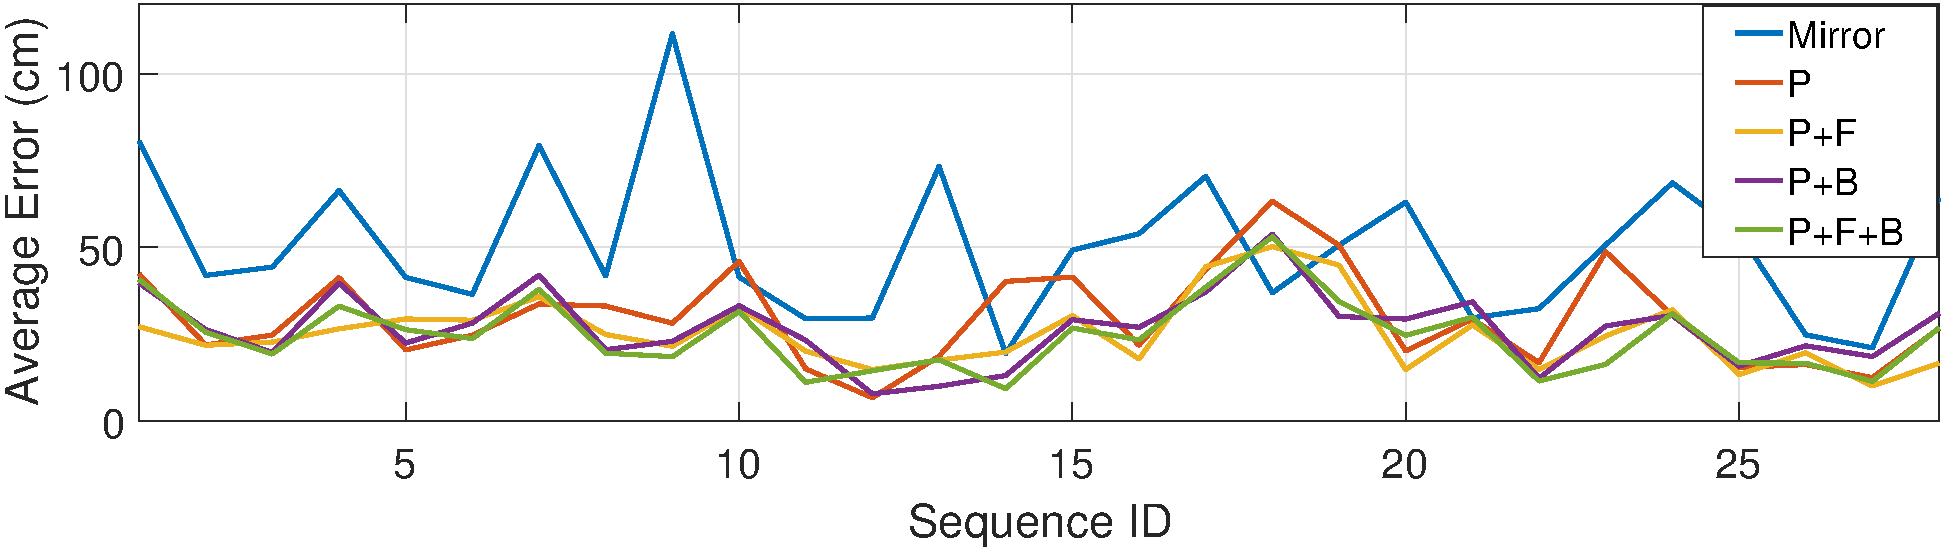
\includegraphics[width=\linewidth]{ssp_fig/cvpr19_predForm}\\
%	\includegraphics[width=\linewidth]{ssp_fig/cvpr19_predBody}
%	\caption{Average error of social formation prediction (top) and body gesture prediction (bottom). $y$-axis for the position errors in centimeters, and $x$-axis is sequence IDs.} %``Mirror" represents the baseline method, and P, F, and B denote Position, Face orientation, and Body orientation, as the input for the prediction.} 
%	\label{fig:predForm_errors}
%\end{figure}



% %Body only
% total_avg_posErr: 29.8286890398, std 13.3812589645
% total_avg_bodyOriErr: 0.263378293988, std 0.124290071428
% total_avg_faceOriErr: 0.327747834313, std 0.129691809416

% %Body + face
% total_avg_posErr: 25.2330815723, std 9.74251270294
% total_avg_bodyOriErr: 0.228412316901, std 0.0890485420823
% total_avg_faceOriErr: 0.303724261948, std 0.116639345884

% %Body + bodyOri
% total_avg_posErr: 26.57, std 10.24
% total_avg_bodyOriErr: 0.22, std 0.08
% total_avg_faceOriErr: 0.30, std 0.10

%While lower error may mean a better result, we may still see whether the prediction behave as human. 
% {\color{red} What happen when the turns are changing }

% {\color{red} Failure cases?}

% Position only, and orientation. 

% W/Wo speaking

% W/Wo body signal

% PCK curves

% Baseline: Trianglular estimation
% Orientation: See always the buyer.

% \begin{figure}
% 	\centering
% 	\includegraphics[width=\linewidth]{plot/cvpr19_predBody}
% 	\caption{Average error of body prediction. $y$-axis for the errors in centimeter, and $x$-axis for the sequences.} 
% 	\label{fig:predBody_errors}
% \end{figure}

\begin{figure*}
	\centering       
	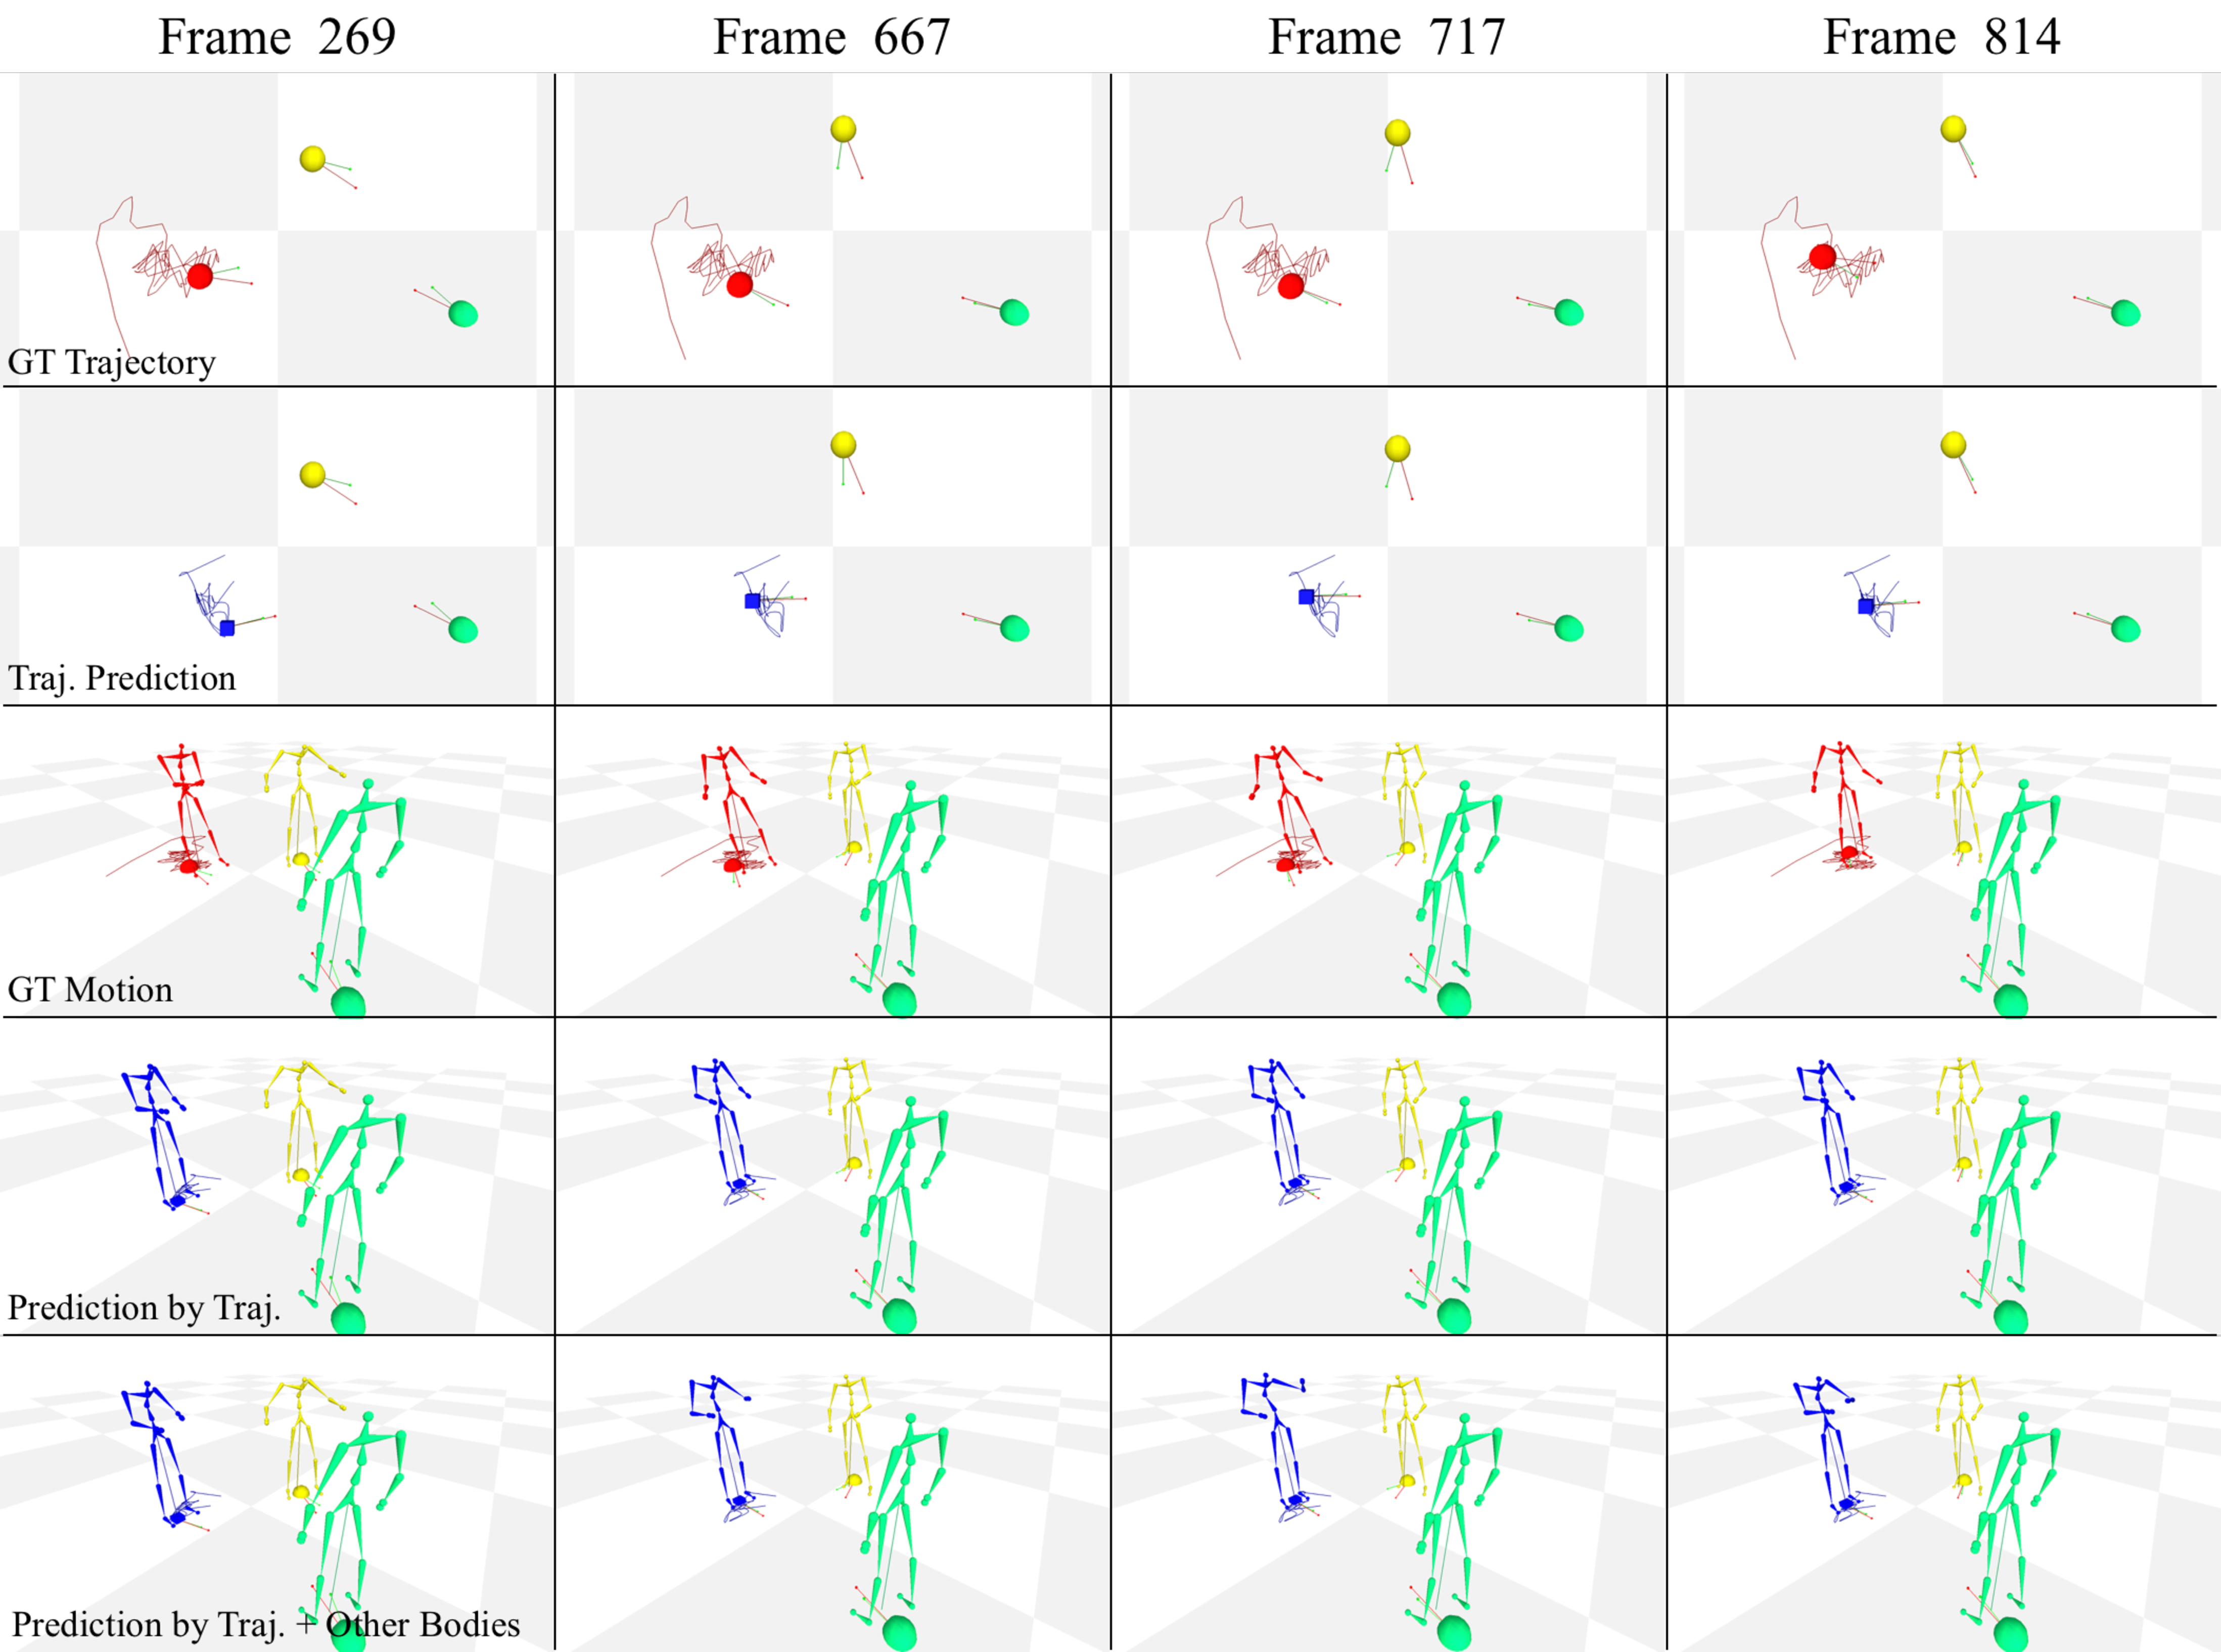
\includegraphics[width=\linewidth]{ssp_fig/qual_170221_b2_group4}
	%	\subfigure[TrajCompares]{\label{Fig:asso_traj}\includegraphics[width=0.5\textwidth]{img/trajCompare}}   
	\caption{An example result of \textit{Social Signal Prediction}. Each column shows scenes at a particular frame. The social signals drawn in green or yellow color are used as the inputs to our method, and blue signals are our social signal prediction results. The signals drawn in red are the ground truth. (First row) The ground truth social formations are shown from a top view, where the target person is shown as red spheres along with trajectories (red curves), face orientation (green arrows pointing from the spheres), and body orientations (red arrows from the spheres). (Second Row) The predicted locations (blue cubes), trajectories (blue curves), face orientations (green arrows), and body orientations (red arrows) are shown. (Third row) The ground-truth 3D body poses of the target person are shown. (Fourth row) We predict the 3D motion from the estimated 2D trajectory of the target person. (Fifth row) We use the body motion of other subjects to predict the upper body motion of the target person, which are combined to the leg body motions estimated from the trajectories.} 
	\label{fig:qualitative}
\end{figure*}

\begin{table}[t]
	\centering
%	\footnotesize
	%\caption{Social Body Gesture Prediction Errors}
	\begin{tabular}{c| c| c}
		
		\hline
		%Types & Avg. dist. (cm) & Std.(cm) & Min dist. (cm)  & Max dist. (cm)\\
		Types & Avg. Joint Errors (cm) & Std.\\
		\hline
		%Mirroring buyer & 11.60 &2.70\\
		%\hline
%		Mirroring input seller & 10.86 &2.49\\
%		\hline
		Mean Pose \underline {\textbf{7.83}} & 2.33\\
		\hline
		Traj2Body & 8.31 & 2.26\\
		\hline
		% 		body2Body & 8.19 (2.01)\\
		Body2Body & 8.72 & 2.00\\
		\hline
		% 		body2Body & 8.19 (2.01)\\
		Traj2Body (lower body) + Body2Body (upper body) & 8.61  & 1.84\\
		\hline
	\end{tabular}
	\caption{Social Body Gesture Prediction Errors (cm). Body orientation and face orientation are computed between estimated and GT unit vectors (need to be fixed) \label{table:predBody_errors}}
\end{table}



\begin{table}[t]
	\centering
	%	\footnotesize
	\begin{tabular}{l| l}
		\hline
		%Types & Avg. dist. (cm) & Std.(cm) & Min dist. (cm)  & Max dist. (cm)\\
		Input Signal & Accuracy\\
		\hline
		\hline
		Ground-truth Own Body & 79.94 \% \\       %new
				\hline
		Ground-truth Other Seller's Body & 75.28 \% \\       %new
		\hline
		\hline
		Mean Pose & 51.03\% \\       %new
				\hline
		Traj2Body & 51.42\% \\       %new
				\hline
		Body2Body & 52.97\% \\       %new
				\hline
		Body2Body+Traj2Body & 52.78\% \\       %new
				\hline
		Face2Body & \underline {\textbf{67.68}}\% \\       %new
				\hline
		Face2Body+Traj2Body & 66.60\% \\       %new
		\hline
	\end{tabular}
	\caption{We evaluate the speaking status of predicted models to quantitatively measure the quality of them. This table shows speaking status prediction accuracies, where the speaking status is predicted from the synthesized body motions from the specified sources.}
\end{table}



\subsection{Body Gestures Prediction}

We predict body motion of the target person by three methods: traj2body, body2body, and face2body. In the ``traj2body" method, the body motion is directly regressed from the estimated social formation (location and orientation) of the target person. This method shows leg motions following the trajectory movements, but has minimum upper body motion. Examples are shown in the fourth row of Fig.~\ref{fig:qualitative}. In ``body2body" method, we predict the target person's body motion by using other subjects' body motion as input. This motion does not take into account the global formation cues, but shows more dynamic body motions by responding to other subjects' motion. We can combine both methods, by merging the formation and leg motion from the first method to the upper body motion from the second method. Examples are shown in the fifth row of Fig.~\ref{fig:qualitative}. In the ``face2body" method, we use other seller's face motion as a source to predict the body motion of the target person. Similarly, we can combine this output with the leg motion of ``traj2body" method. The final prediction results show human-like social behaviors including location, body and face orientation, leg motion, and hand gestures. 

We evaluate the prediction performance of body gesture using the common L2 distance and our proposed speaking status based metric. We consider a baseline method, ``Mean Pose", by computing the average posture of all training data and constantly use it as prediction output. As shown in Table~\ref{table:predBody_errors}, the L2 error of this baseline shows the best performance, although this motion is not realistic and not suitable for the social scene.

In our new metric, we first predict the speaking status from the synthesized motion. We use the pre-trained classifier that takes own body signals as input. And then compute the accuracy by comparing the current speaking status with ground truth. This metric mainly checks the turn-taking property, penalizing the output if the synthetic motion does not follow this social rules. As described in section~\ref{section:evaluation}, the mean pose shows almost a chance level accuracy, since the motion looks not speaking at all. The prediction by ``body2body" method shows a better performance, but we found the timing of the output motion is not accurate. ``face2face" method shows the best performance, since the face cues provide a strong clue to determine the speaking timing, as demonstrated in Table~\ref{table:speaking_class}. As shown in this result, our social signal prediction method shows a reasonable performance in modeling the dynamics of social signals, and our evaluation method can be used to quantify the output.


%The final outputs predict more natural social behaviors than other baselines, satisfying most of the noticeable social rules in the scenes (distance, orientation, leg and root movement, and natural hand motions). Our results are best seen in the supplementary videos. However, the quantitative errors tend to be higher, as shown in Table~\ref{table:predBody_errors} and Figure~\ref{chapter:predBody_errors}. Notably, the average pose computed from the training set shows the best performance. This is because the error metric computing the 3D errors from the ground-truth cannot fully evaluate how natural the motion appears. %Given the similar social signal inputs, there are diverse possible suitable human motions, and a better evaluation method is required to consider this.%  the quality of social signal prediction.% and it should be related to a 

% {\color{red} Qualitative example where turn taking is captured?}

% \noindent \textbf{Direct Regression from Social Formations:}
% We can directly regress from the predicted 2D formation output.  

% PCK curves 
% Per joint


% \textbf{Regression from Richer Input:}
% We use other skeletons and input and see any improvement. 

% Compared to the direct regression. 
% {\color{red} Any semantic improvement which is not captured by numbers?}

% Any good way to evaluate realistic human motion???


% \subsection{Quantifying Social Signal Importance}



% \subsection{Correlation between Body, Face, and Hands}

% We use all body parts for communication where each part plays a role to send some specific signals. Unfortunately, these roles are also poorly understood. In this section, we investigate whether there exists patterns or strong correlations among parts. We study this by predicting a missing part given other body parts. 

% Body2face, face2body

% \subsection{Face and Hands signals}